% Options for packages loaded elsewhere
\PassOptionsToPackage{unicode}{hyperref}
\PassOptionsToPackage{hyphens}{url}
%
\documentclass[
  12pt,
]{article}
\usepackage{lmodern}
\usepackage{amssymb,amsmath}
\usepackage{graphicx}
\usepackage{ifxetex,ifluatex}
\ifnum 0\ifxetex 1\fi\ifluatex 1\fi=0 % if pdftex
  \usepackage[T1]{fontenc}
  \usepackage[utf8]{inputenc}
  \usepackage{textcomp} % provide euro and other symbols
\else % if luatex or xetex
  \usepackage{unicode-math}
  \defaultfontfeatures{Scale=MatchLowercase}
  \defaultfontfeatures[\rmfamily]{Ligatures=TeX,Scale=1}
  \setmainfont[]{Hoefler Text}
  \setsansfont[]{Gill Sans}
\fi
% Use upquote if available, for straight quotes in verbatim environments
\IfFileExists{upquote.sty}{\usepackage{upquote}}{}
\IfFileExists{microtype.sty}{% use microtype if available
  \usepackage[]{microtype}
  \UseMicrotypeSet[protrusion]{basicmath} % disable protrusion for tt fonts
}{}
\makeatletter
\@ifundefined{KOMAClassName}{% if non-KOMA class
  \IfFileExists{parskip.sty}{%
    \usepackage{parskip}
  }{% else
    \setlength{\parindent}{0pt}
    \setlength{\parskip}{6pt plus 2pt minus 1pt}}
}{% if KOMA class
  \KOMAoptions{parskip=half}}
\makeatother
\usepackage{xcolor}
\IfFileExists{xurl.sty}{\usepackage{xurl}}{} % add URL line breaks if available
\IfFileExists{bookmark.sty}{\usepackage{bookmark}}{\usepackage{hyperref}}
\hypersetup{
  pdftitle={English Department Undergraduate Courses},
  hidelinks,
  pdfcreator={LaTeX via pandoc}}
\urlstyle{same} % disable monospaced font for URLs
\usepackage[paperheight=8.5in,paperwidth=5.5in,bottom=0.75in,top=0.75in,left=0.5in,right=0.5in]{geometry}
\setlength{\emergencystretch}{3em} % prevent overfull lines
\providecommand{\tightlist}{%
  \setlength{\itemsep}{0pt}\setlength{\parskip}{0pt}}
\setcounter{secnumdepth}{-\maxdimen} % remove section numbering
\ifluatex
  \usepackage{selnolig}  % disable illegal ligatures
\fi


\newlength{\cslhangindent}
\setlength{\cslhangindent}{1.5em}
\newlength{\csllabelwidth}
\setlength{\csllabelwidth}{3em}
\newlength{\cslentryspacingunit} % times entry-spacing
\setlength{\cslentryspacingunit}{\parskip}
\newenvironment{CSLReferences}[2] % #1 hanging-ident, #2 entry spacing
 {% don't indent paragraphs
  \setlength{\parindent}{0pt}
  % turn on hanging indent if param 1 is 1
  \ifodd #1
  \let\oldpar\par
  \def\par{\hangindent=\cslhangindent\oldpar}
  \fi
  % set entry spacing
  \setlength{\parskip}{#2\cslentryspacingunit}
 }%
 {}
\usepackage{calc}
\newcommand{\CSLBlock}[1]{#1\hfill\break}
\newcommand{\CSLLeftMargin}[1]{\parbox[t]{\csllabelwidth}{#1}}
\newcommand{\CSLRightInline}[1]{\parbox[t]{\linewidth - \csllabelwidth}{#1}\break}
\newcommand{\CSLIndent}[1]{\hspace{\cslhangindent}#1}

\usepackage{multicol}


\title{``vellum in war time'': Playing with MJP Data}
\author{}
\date{}

\begin{document}

\begin{quote}
It is important that you should send the edition on extra fine paper to
a certain sort of person. Only a finely got up magazine will strike the
eye in certain districts. The rough paper is good enough for the other
people whose names I've sent you. The swells in Paris won't expect
vellum in war time. ---Ezra Pound to Margaret Anderson, May 5, 1917 (43)
\end{quote}

\begin{quote}
there is a certain type of mind that worries about such things. Quant a
moi, I am more concerned with what people say than with the ink it is
written in. ---Pound to Anderson, May 24, 1917 (55)
\end{quote}

\begin{quote}
``the public'' likes a lot of paper for its money ---Pound to Anderson,
November 12, 1917 (151)
\end{quote}

\hypertarget{playing-with-data}{%
\subsection{Playing With Data}\label{playing-with-data}}

The most exciting thing I learned at
\href{http://msa.press.jhu.edu/conferences/msa13/index.html}{MSA 13} was
that the Modernist Journals Project has made some of its data available
for tinkerers to play with; specifically, the full text and metadata
records for five little magazines: \emph{The Freewoman}, \emph{The New
Freewoman}, \emph{The Egoist} (these latter three represent a sort of
single, permutating evolution), \emph{Others}, and \emph{The Little
Review}.

The full-text is available in \emph{very} lightly marked up TEI files
(for nearly all purposes, you'd be best just stripping out the tags and
treating it as plain-text) and metadata about the journals in separate
\href{http://www.loc.gov/standards/mods/}{MODS} files (the acronym is
wonderfully appropriate). Their new demo site,
\href{http://dev.stg.brown.edu/projects/mjplab/}{MJP Lab}, shows some of
the things they've been doing; and if you want to try some things
yourself, you can grab the data yourself at the
\href{http://sourceforge.net/p/mjplab/home/Home/}{MJP sourceforge page}

I was eager to get home and start playing; this post represents a
belated first stab at some tinkering, in the hope of helping to start a
conversation about what sorts of neat things we can do with this stuff;
because if we can do some neat stuff with this stuff, hopefully the good
folks at the \emph{MJP} will continue this trend, and make their other
material available. In this post I focus chiefly on a pretty crude unit
of analysis---length.

\hypertarget{paper-shortage}{%
\subsection{Paper Shortage}\label{paper-shortage}}

Why would the length of a little magazine change? It was
\href{http://twitter.com/tcarmody}{Tim Carmody} who first suggested to
me that a paper shortage during World War I might have had an important
impact on the publishing of modernism. I can't now locate the tweet, or
series of tweets, where Tim first made this suggestion, but the
inspiration with which I'll toy for a while here is entirely
Tim's---only the mistakes and bad code are mine.

It is hard to get the news from poems; but its harder to get the history
of paper from books. Histories of paper are often histories of
paper-making technologies. (I'd be very grateful if anyone has a good
recommendation of a book addressing the history paper, including paper
costs and shortages, etc in the early twentieth century.) In desperation
you might turn to Google Books and find
\href{http://books.google.com/books?id=cP8fAQAAMAAJ}{Paper}, a
periodical ``devoted to the manufacture, sale, and use of pulp and
paper,'' which reports, in September 1914 that ``So far as can be
observed by surface inspection the war has not affected manufacturing
conditions so much as was expected a month ago. However, every day that
passes brings the time of serious affection nearer.'' By December 1914,
``the effects of the European war upon the paper industry was
demonstrated to be quite important the other day\ldots{}''

In a tweet I've long since lost, Tim points to
\href{http://books.google.com/books?id=GZMNYLgd5X4C\&pg=PA133\&lpg=PA133\#v=onepage\&q\&f=false}{this}
passage from an essay on Joyce which Pound published in 1918: ``Despite
the War, despite the paper shortage\ldots{} there is a new edition of
James Joyce's `A Portrait of the Artist'\,'' (\emph{Pound/Joyce} 133).

So certainly some concern exists (at least in America) about the
availability of paper.

Ezra Pound's letters to Margaret Anderson (editor of the \emph{Little
Review}) are interesting but never quite so clear (and here follows a
bunch of quotations from the letters; feel free to move along). In a
letter from which I quoted at the head of the this post, Pound writes
that ``Failing an increase in size, an improvement in paper
\textless(even a slight imp)\textgreater{} would make a fuller use of
the smaller font of type less disagreeable. That might be an
intermediate move.'' That Pound is talking about an increase in
\emph{length} is clear from the next comment that ``We might aim for 48
pages by September'' (46). An editorial note to this letter (citing, in
turn, a letter from Donald Gallup) explains that ``perhaps as many as
twenty-five copies\ldots{} of some issues of the \emph{LR} were printed
on high quality paper. This fact, Gallup notes, 'is especially important
because the''rough'' paper was of such bad quality that many runs of
\emph{The Little Review} have crumbled away and many libraries\ldots{}
have only microfilm.'' (47). A month later Pound wants ``to go to 64
pages just as soon as it can be managed.'' Throughout his letters to
Anderson, Pound can be seen weighing the cost of paper against other
factors; Yeats, for instance, must have a copy printed on high quality
paper (``he'll fuss and lose interest if he sees his poems on cheap
paper'' 55); but it is equally important to ``get a good deal of actual
matter into Oct, Nov, Dec.~EVEN if you have to use newspaper paper''
(104). (Here as so often, one longs to have Anderson's half of the
correspondence.) In a letter from December 1917, Pound insists that
``official stationary for official business is pure swank. AT the
present price of paper!!!'' (167), suggesting that indeed paper during
the period of the war was getting dear.

So, did the war create a paper shortage which impacted little magazines
in significant ways?

\hypertarget{looking-at-the-data}{%
\subsection{Looking at the Data}\label{looking-at-the-data}}

However dry this question may seem, it has the advantage of being
answerable with the MODS data. Each issue in the \emph{MJP} has its own
MODS record containing metadata which includes the journal title, titles
and authors of the texts contained in that issue, a date of publication,
and a description of the physical object, including number of pages.

For example, here is the beginning of the record for the first issue of
the \emph{Egoist}:

\{\% highlight xml \%\}

The Egoist An Individualist Review Vol. 1, No.~1\\

Marsden, Dora editor

periodicals

Egoist:1:1

enk London The Egoist, Ltd. 1914-01-01

20 p.; 31.5 x 21 cm reformatted digital

\{\% endhighlight \%\}

To get the information we want, we just need a little XSLT. Simple,
right? Well, I don't really know XSLT, but google and persistence will
yield answers if not elegance:

\{\% highlight xslt \%\}

:: :: ::

\{\% endhighlight \%\}

The ``xmlns:mods=''http://www.loc.gov/mods/v3'' line is necessary to let
XSLT know about the MODS namespace (you get an error otherwise; trust
me); we declare an output method of text (we'll be essentially
generating an self-styled text data file; you could output xml or html).
Then we match the root element, and select just the data we want, in
this case the journal title, the volume and number information, the
date, and then the ``extent'' which is the size and number of pages. If
you've noticed that ugliness in the last select statement, it's because
I'm using the \emph{concat{[}enate{]}} function to manually add a
newline character entity at the end, so that we get one line of output
per issue. You may also have noticed that each of these fields is
separated by a double colon. The more obvious field delimited---a
comma---would cause a problem here since the ``extent'' field, for
instance, has commas within it. So the double colons will make life
easier.

(Yeah, this is ugly; if you have tips on a more elegant way of doing
this, I'm all ears).

Use xsltproc with this stylesheet on the MODS file for the first issue
of the Egoist and the output looks like this:

\{\% highlight xml \%\} Egoist::Vol. 1, No.~1::1914-01-01::20 p.; 31.5 x
21 cm \{\% endhighlight \%\}

But if you've downloaded all the MODS files and unzipped them in a
single directory, then a command like xsltproc extract.xsl *.xml
\textgreater{} total.dat will get the data from everything; and indeed,
you can find all data from all the freely accessible journals in a
\href{https://docs.google.com/spreadsheet/ccc?key=0Aqxybvy6W0jedE5QczhNYTdVVXFua2k3cnZtcmh2SUE}{Google
Doc} (note that the Google Doc importer seems to have gotten a bit
confused by the dates).

This work flow makes it easy to add new data as it becomes available;
just place it in the directory, rerun xsltproc\ldots{} and there you go.

\hypertarget{paper-and-the-war}{%
\subsection{Paper and the War}\label{paper-and-the-war}}

You could just peruse this list to see that, for example, \emph{The
Egoist} does seem to get shorter during the war years. In late 1914 it
drops from 20 to 16 pages, and then drops again to 12 pages in 1918
before returning to 16 pages for its last year in print, 1919. (Maybe
everyone already knew this; maybe, among specialists in \emph{The
Egoist} this shortening has a well known explanation. Anyone?)

Since I'm used to doing things with
\href{http://processing.org}{processing}, I'll offer this rather
rudimentary visualization of changes in length of all five journals for
which data is available. (I'm doing something wrong in the main draw()
loop so that the fonts are coming out ugly, but you get the idea):

\par\begin{figure}\centering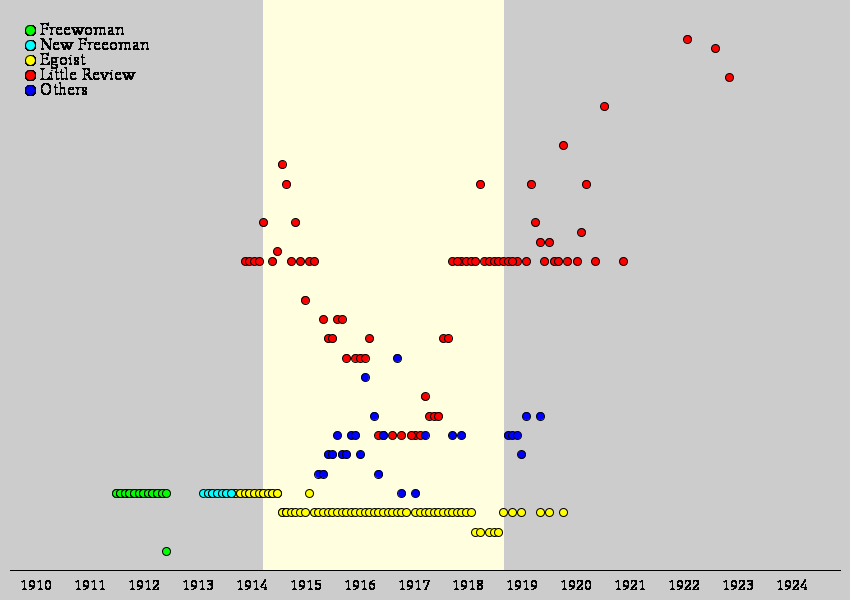
\includegraphics[width=\columnwidth]{_images/mjp-mods.png}\caption{}\end{figure}

Only three of the five journals are being published during the First
World War. Both \emph{The Little Review} and \emph{Others} are not
nearly so regular as \emph{The Egoist}. Nevertheless, if you tilt you
head, there does seem to be a general decline in journal length during
the war; but really we'd want more data before we made anything of this.

\hypertarget{images}{%
\subsection{Images}\label{images}}

Of course, one of the reasons I wanted to share even these rather
incomplete and ugly results is that once you start tinkering, its hard
to stop. Consider this: if paper is getting expensive, you might begin
to try to fit more on a single page. Just to see whether I could do it,
I decided to try to compare the page layouts of \emph{The Egoist} when
it was a full 20 pages (in 1914) to the shorter, 12 page \emph{Egoist}
of 1915. (I focus on \emph{The Egoist} here because the shifts in its
length created a clear opportunity for comparison.)

There would be other ways to look into this (including doing word counts
on the full text files). But here is one thing you might try: first,
grab the complete PDFs of a few issues from Vol 1 (1914) and Vol 5
(1915) of \emph{The Egoist}. Without too much thought I got Vol 1,
issues 1--5 and Vol 5, issues 1--5. The wonderful tool
\href{http://www.pdflabs.com/tools/pdftk-the-pdf-toolkit/}{pdftk} has a
``burst'' function will separate a pdf into individual pages. These, in
turn can easily be turned into individual PNG page images, using
\href{http://www.imagemagick.org/script/index.php}{imagemagick}. Indeed,
imagemagick is really the secret sauce here.

After that, we have two directories containing page images, one for the
Vol 1 issues and one for the Volume 5 issues. Imagemagick has a
\href{http://www.imagemagick.org/Usage/layers/\#evaluate-sequence}{function
that will ``average''} a set of images; imagine, for instance, taking 50
images setting each to 2\% transparency and then stacking them all
together so that you have a single page. The trick is that the images
have to all be the \emph{exact} same size for the average function to
work (it is comparing the same pixel location across multiple images, so
size is key). That is easy enough with imagemagick as well. To get all
the images in a directory the same size: convert *.png -size 620x960!

The trick to that command is the exclamation point at the end (which has
to be escaped in most circumstances, hence the slash) which tells
imagemagick to \emph{not} preserve the image's original aspect ratio.
This is crucial because for average to work the images must all be
identical (otherwise, after watching your CPU chug away at 100\% for
five minutes, it will throw an error and leave a bunch of useless files
in your directory). This will introduce some very minor distortion into
the images, but it is a small price to pay (so long as you're comparing
images which are all \emph{very nearly} identical in size to begin
with). Once you've got your directory of images, all properly resized,
here is the magic command (thanks to the
\href{http://www.imagemagick.org/discourse-server/viewtopic.php?f=1\&t=19754}{kind
folks} on the imagemagick forum):

convert Vol1*.png -evaluate-sequence mean average\_page.png

When all that's done you get something which looks like this:

\par\begin{figure}\centering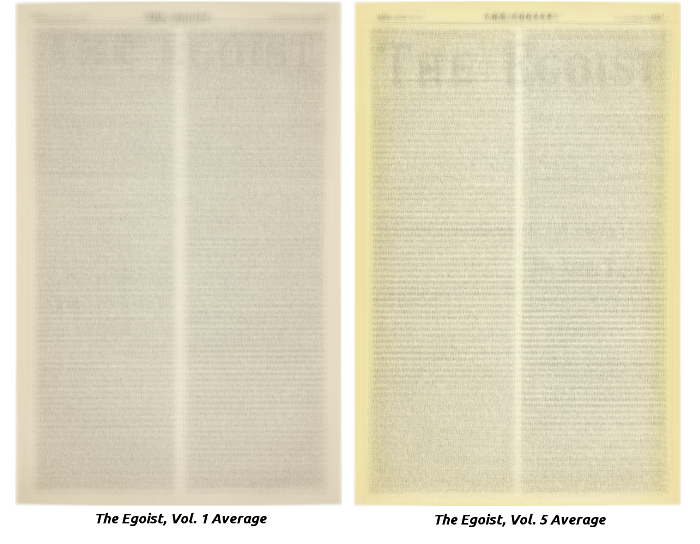
\includegraphics[width=\columnwidth]{_images/comparison_sm.png}\caption{}\end{figure}

Nothing revolutionary; but sort of interesting. Note, for instance, that
you can more easily make out the ``Egoist'' logo in the Volume 5 image,
which makes sense---since each issue of the Volume 5 is shorter, the
title page represents a larger proportion of the total set of pages.

\par\begin{figure}\centering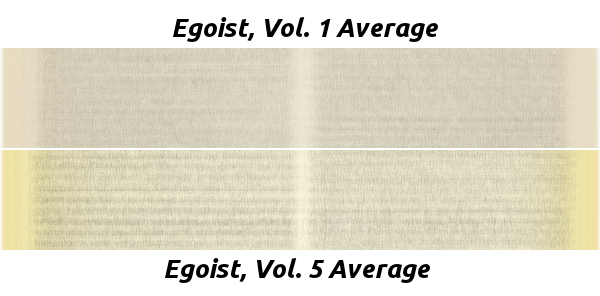
\includegraphics[width=\columnwidth]{_images/alley_comparison.png}\caption{}\end{figure}

What \emph{may} be interesting is that the alley (the gap between the
two columns of text) seems to be narrower in Volume 5 than in Volume 1
(it is a little difficult to see here; check the originals below if
you're curious; maybe I'm seeing things); does this suggest that rising
paper costs during the war folks to squeeze more text onto each page?
(What about the margins? It is hard to tell, but the margins too may be
slightly smaller in the Volume 5 image).

If you want to can see the original averages:
\href{/images/Vol1-average.png}{Volume 1} and
\href{/images/Vol5-average.png}{Volume 5}. \textbf{Warning, the files
are \textasciitilde2.7 megabytes}.

When I get a moment, I'll be trying to do some other things with this
data. More data from other little magazines might shed light on changes
in the length of little magazines during the war, at which point it
would make sense to return to the journals themselves.

\hypertarget{concluding-methodological-postscript}{%
\subsection{Concluding Methodological
Postscript}\label{concluding-methodological-postscript}}

I've made this point before, but the kludgy, tinkering series of things
I did with the data is not the product of using any one tool. PDFTK,
ImageMagick, processing, and XSLT were all thrown together. Rather than
trying to imagine a single tool to rule them all, I think this sort of
flexible tool chain is really the way to go. A little programming, a
little data manipulation, and some command line tools can really go a
long way.

\hypertarget{works-cited}{%
\subsubsection{Works Cited}\label{works-cited}}

\begin{itemize}
\tightlist
\item
  Pound, Ezra. \emph{Pound / The Little Review: The Letters of Ezra
  Pound to Margaret Anderson}. Ed. Thomas L. Scott, et al.~New York: New
  Directions, 1988. Print.
\end{itemize}

\end{document}
